\documentclass[xcolor=dvipsnames]{beamer}

\usepackage[italian]{babel}
\usepackage[utf8]{inputenc}
\usepackage[T1]{fontenc}
\usepackage{color}
\usepackage{hyperref}
\usepackage{graphicx}
\usepackage{floatflt}
\usepackage{float}
\graphicspath{{images/}}
\usepackage{eurosym}
\usepackage{colortbl}
\usepackage{color}
\raggedbottom
\usetheme[currentsubsection]{PaloAlto} 
\usecolortheme{seahorse}
\setbeamertemplate{footline}[frame number]
\setbeamertemplate{items}[ball] 
\setbeamertemplate{blocks}[rounded][shadow=true] 
\title{CPNetSolver}
%\subtitle{}
\author{Francesco Burato, Simone Carriero}
\institute[UNIPD]{
  Dipartimento di Matematica\\
  Università degli Studi di Padova\\[1ex]
  %\texttt{lambdaset@gmail.com}
}
\date{12 Settembre 2013}
\newcommand{\firstFrame}[1]{
\begin{frame}
  \begin{block}{CPNetSolver}
    \begin{center}
    #1
    \end{center}
   \end{block}
\end{frame}
}
\begin{document}

%--- the titlepage frame -------------------------%
\begin{frame}[plain]
  \titlepage
\end{frame}

\section{Introduzione}
\begin{frame}{Introduzione}

Cos'è CPNetSolver
\begin{itemize}
  \item risoluzione di CP-Net
  \item visualizzazione grafo dell'ordine degli assegnamenti
  \item accetta anche CP-Net cicliche
\end{itemize}
\end{frame}

\begin{frame}{Introduzione}

Funzionamento:
\begin{itemize}
  \item accettazione CP-Net in input
        %(DIRE:grammatica pross. slide)
  \item conversione da CP-Net a CSP
  \item calcolo e visualizzazione soluzioni ottime
  \item generazione e visualizzazione grafo dell'ordine degli assegnamenti
\end{itemize}

Idea iniziale:
\begin{itemize}
  \item strumento didattico!
  %(DIRE:in ciascun momento si può cambiare la CP-Net
  %corrente e vedere come cambiano le soluzioni e gli ordinamenti)
  
\end{itemize}
\end{frame}

\begin{frame}[fragile]{Introduzione}

Grammatica
\begin{itemize}
\item
\begin{verbatim}
var X dependsOn={}
dom={x,!x}
:x>!x

var Y dependsOn={}
dom={y,!y}
:y>!y

var Z dependsOn={X,Y}
dom={z,!z}
x,y:z>!z
x,!y:!z>z
!x,y:!z>z
!x,!y:!z>z
\end{verbatim}
\end{itemize}
\end{frame}


\section{Progettazione}
\begin{frame}{Suddivisione architetturale}
\begin{itemize}
  \item package \texttt{constraintobj}
  \item package \texttt{solver}
  \item package \texttt{gui}
\end{itemize}
\end{frame}

\begin{frame}{Rappresentazione dei domini}

\begin{itemize}
  \item class Domain
  \begin{itemize}
    \item[-] accepted: Set[String]
    \item[+] contains(elem: String): Boolean
  \end{itemize}
\end{itemize}
\end{frame}

\begin{frame}{Rappresentazione dei vincoli}
\begin{itemize}
  \item class Constraint
  \begin{itemize}
    \item[-] vars: Array[String]
    \item[-] accepted: List[Array[String]]
    \item[+] projection(variable: String): Set[String]
    \item[+] reduction(variable: String, value: String): Constraint
  \end{itemize}
\end{itemize}
\end{frame}

\begin{frame}[fragile]{Esempio di oggetto constraint}
\begin{verbatim}
c = Constraint(vars     =>  [X, Y, Z]
               accepted => [[0, 0, 1],
                            [0, 1, 1],
                            [0, 1, 0]])
                            
c.projection(X) = [0]
c.projection(Y) = [0, 1]

c.reduction(Y,1) = Constraint(vars     =>  [X, Y, Z]
                              accepted => [[0, 1, 1],
                                           [0, 1, 0]])
\end{verbatim}  
\end{frame}

\begin{frame}{Rappresentazione degli ordini - 1}
\begin{itemize}
  \item class Order
  \item \textbf{Rappresentazione ad albero}: nodi interni per gli assegnamenti, foglie per gli ordini
  \pause
  \item class Comparator per l'accesso
  \item Complessità dipendente dalla \textbf{ricerca nei nodi interni}
  \begin{itemize}
  	\item Ricerca lineare: $O(|dom(V_1)|+\ldots+|dom(V_n)|)$
  	\item Ricerca binaria: $O(log(|dom(V_1)|\cdot \ldots \cdot|dom(V_n)|))$
  	\item Tabella hash:    $O(1)$
  \end{itemize}
\end{itemize}
\end{frame}

\begin{frame}{Rappresentazione degli ordini - 2}
Esempio

\texttt{var A dependsOn=\{B,C,D\}}  \texttt{dom=\{...\}}\\
\texttt{var B dependsOn=\{\}}       \texttt{dom=\{$b$,$\overline{b}$\}}\\
\texttt{var C dependsOn=\{\}}       \texttt{dom=\{$c$,$\overline{c}$\}}\\
\texttt{var D dependsOn=\{\}}       \texttt{dom=\{$d$,$\overline{d}$\}}\\
\begin{center}
  \begin{figure}[ht]
    \centering
    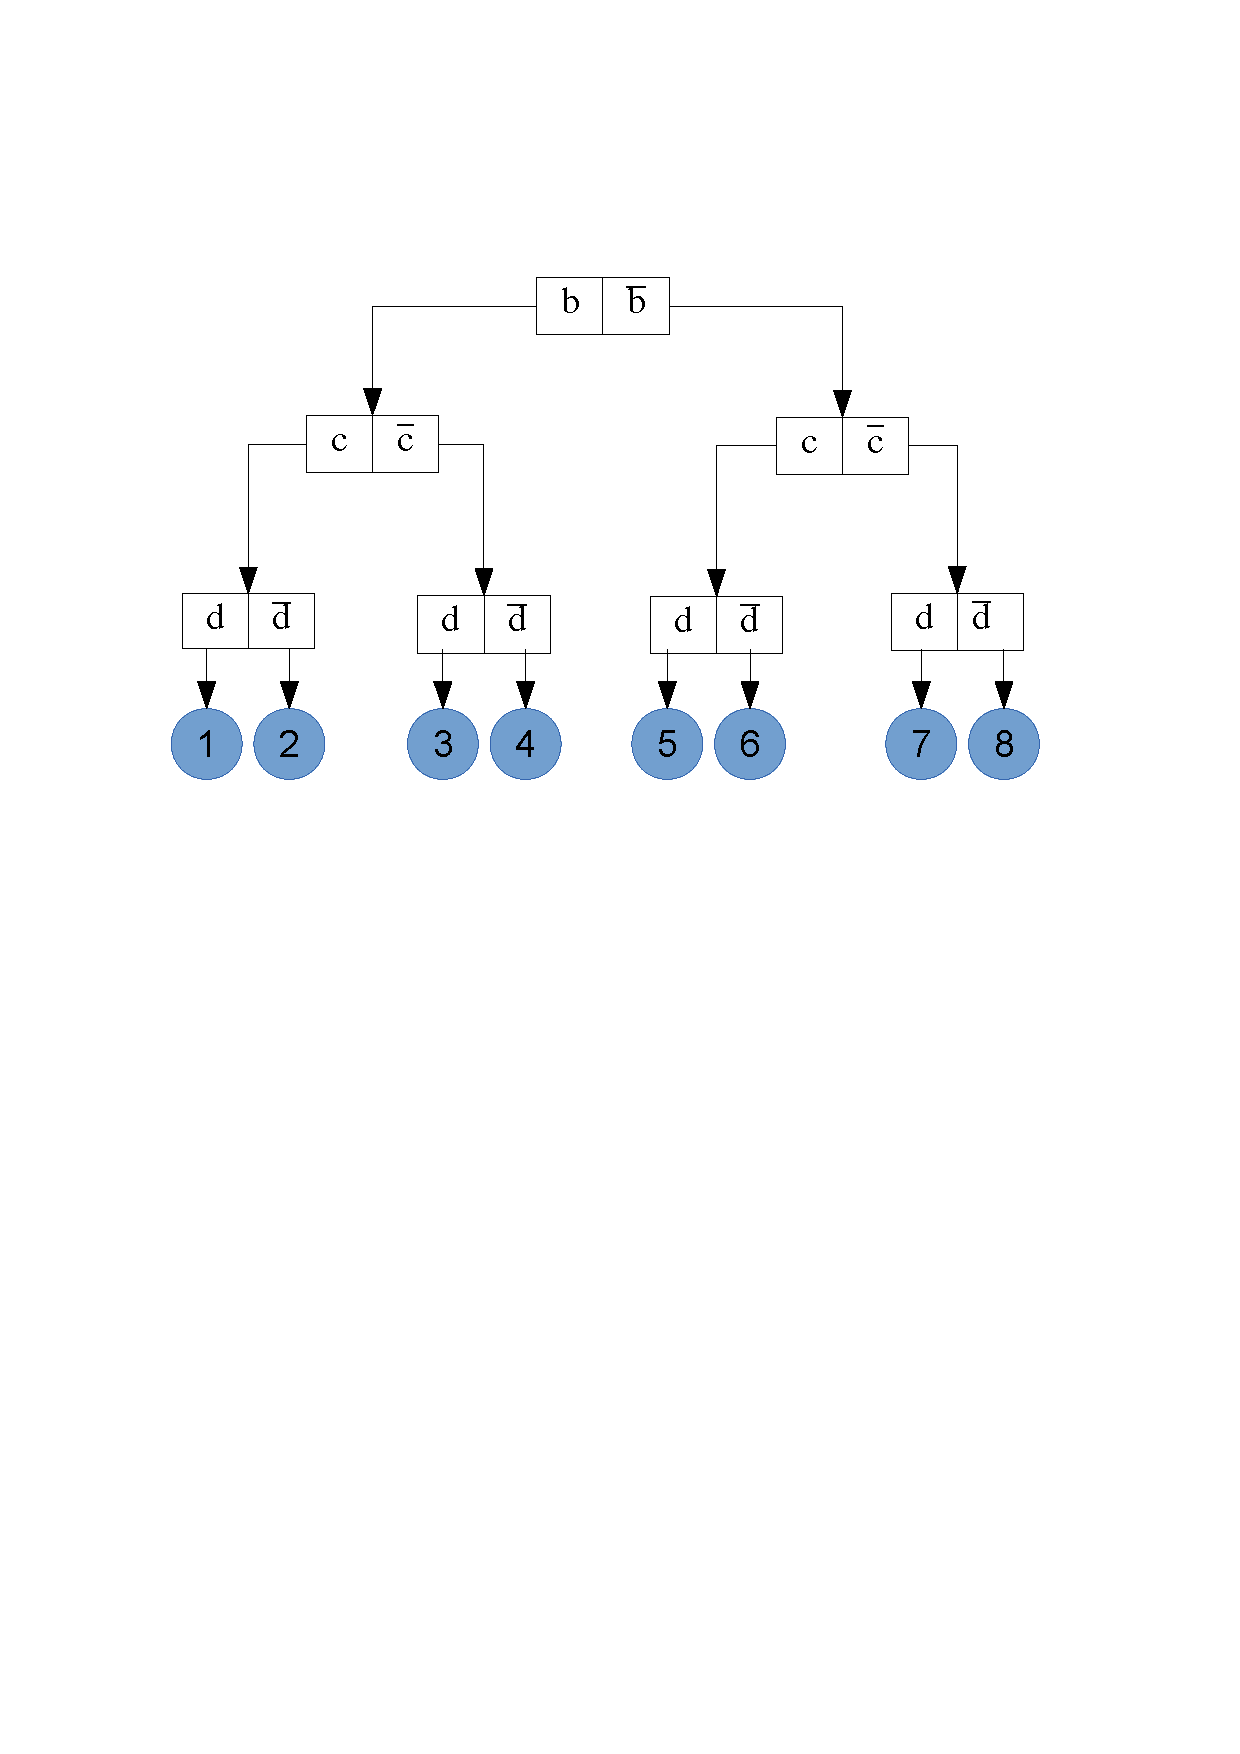
\includegraphics[width=0.5\textwidth]{images/grafo-ordini}
    \caption{\textit{Rappresentazione a grafo di A, B, C, D}}
  \end{figure}
\end{center}
\end{frame}

\end{document}
